\documentclass[10pt,twocolumn]{article}
\usepackage{geometry}
\geometry{verbose,headsep=3cm,tmargin=2.5cm,bmargin=2.5cm,lmargin=2.0cm,rmargin=2.0cm}
\usepackage{graphicx}
\usepackage{xcolor}
\usepackage[font=small]{caption}
\usepackage{cleveref}
\usepackage{amsmath,amssymb,latexsym}
\usepackage{marvosym}
\usepackage{url}
\usepackage{lipsum}
\usepackage{bm}
\usepackage{float}
\usepackage[english]{babel}
\usepackage{hyperref}
\usepackage{epsf}
\usepackage{float}
\usepackage{mathpazo}
\usepackage{pifont}
\usepackage{wrapfig}
\usepackage{multicol}
\usepackage{enumitem}
\usepackage{xcolor}
\usepackage{framed}
\usepackage[utf8]{inputenc}
% Document font:
\usepackage{charter}
\graphicspath{{DWGs/}}

\begin{document}

\twocolumn[{
\begin{@twocolumnfalse}

  \begin{center}
%\textcolor{lgray}
    \vskip-5em

    \hfill
    \fontsize{10}{10}\selectfont {\textit{Bruxelles, November 2018}}

    \vskip2ex
    
	\vspace{5ex}
	
    \fontsize{24}{10}\selectfont {Notes on Dynamic Mode Decomposition}
    
    \fontsize{18}{10}\selectfont {(with some code)}
    
 
      \vspace{1ex}
   \fontsize{10}{10}\selectfont {camillejr.github.io/science-docs}
          
  \noindent%
    
\vskip1ex

{\rule{\textwidth}{0.5pt}}

  \end{center}
  
\vspace{8mm}

\end{@twocolumnfalse}
}]

\setlength{\parindent}{0cm}


\section*{Preface}

\textit{Dynamic Mode Decomposition} (DMD) is a data-driven method of finding low-rank structures in high-dimensional data sets. 

These notes are taken from two lectures on Dynamic Mode Decomposition: [\ref{bib:kutz_1}] and [\ref{bib:kutz_2}] by Prof. Nathan Kutz from the University of Washington.

\,\,

This document is still in preparation.

\tableofcontents


\vspace{10mm}


\section{Description of the system}

We have a system described by a differential equation:

\begin{equation} \label{eq:system_DE}
\frac{d \vec{x}}{dt} = f(\vec{x}, t, \mu)
\end{equation}

The function $f(\vec{x}, t, \mu)$ is a way of \textit{modeling} that system.

We also have \textit{measurements} of the system in different points in space at time $k$, in the form of a vector(s) $\vec{y}_k$:

\begin{equation}
\vec{y}_k = g(\vec{x}_k)
\end{equation}

\begin{wrapfigure}{R}{0.2\textwidth}
\centering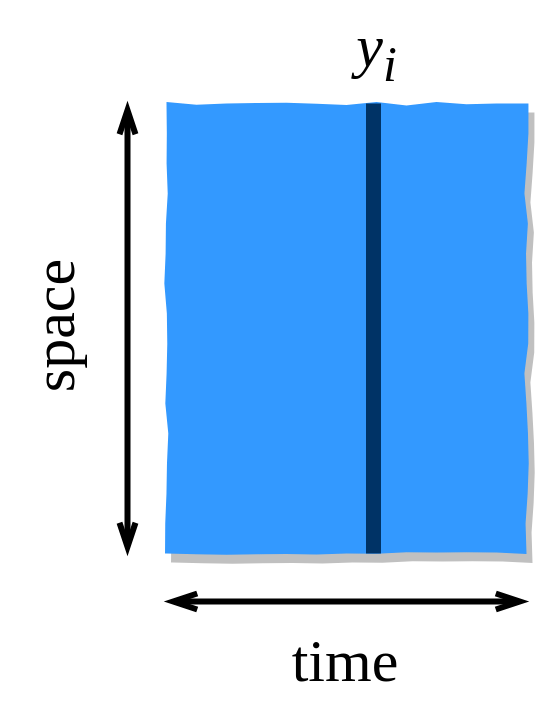
\includegraphics[width=3.5cm]{data-matrix.png}
\caption{Data matrix with measurements of the system.}
\label{fig:data-matrix}
\end{wrapfigure}

where $\vec{x}_k$ is the quantity of interest that we are aiming at measuring. The fact that we might not be able to measure it directly is accounted for by some function $g()$ (although it might happen that $\vec{y}_k = \vec{x}_k$, meaning that we are able to measure $\vec{x}_k$ directly).

Notice, that for measurements at many moments in time, we may stack all the collected vectors $\vec{y}_i$ for different times $i$ to create a matrix whose columns represent time snapshots and whose rows represent position in space.

\section{Linear dynamical systems}

We are from now interested in systems where the governing equation from eq.(\ref{eq:system_DE}) is not known (in other words, the function $f$ is unknown) and we solely rely on measurements of the system which, in general, form a high-dimensional data set.

In the Dynamic Mode Decomposition we approximate that data set by a linear dynamical system of the form:

\begin{equation} \label{eq:system_linear}
\frac{d \vec{x}}{dt} = \bm{A} \vec{x}
\end{equation}

This is in fact a very handy approximation since we are able to write down exact solutions to linear systems.

Once we assume that the general solution is of the form:

\begin{equation} \label{eq:general_solution}
\vec{x} = \vec{v} e^{\bm{\lambda} t}
\end{equation}

to obtain the parameters we effectively solve the eigenvalue problem:

\begin{equation} \label{eq:eigenvalue_solution}
\bm{A} \vec{v} = \bm{\lambda} \vec{v}
\end{equation}

The exact solution to the linear system from eq.(\ref{eq:system_linear}) is:

\begin{equation} \label{eq:soln_exact}
x = \sum_{j = 1}^{n} b_j \phi_j e^{\lambda_j t}
\end{equation}

For a reader who is now shaky about how this solution was derived, more can be found in appendix \ref{app:A}. 

\section{Dynamic Mode Decomposition theory}

\subsection{Exact DMD}

For the moment, we assume that we can measure the system directly, that is we measure $\vec{y}_i = \vec{x}_i$. Moreover, we assume that our data is collected in equal\footnote{Which is indeed a special case for real life measurements. Check section \ref{sec:view} for more information.} time steps $\Delta t$. The measurements are combined inside a large matrix $\bm{X}$ where each of its columns represents one time snapshot:

\begin{equation} \label{eq:X}
\bm{X} = 
\begin{bmatrix}
    \vec{x}_1 & \vec{x}_2 & \vec{x}_3 & \dots & \vec{x}_{m}
\end{bmatrix}
\end{equation}

We split the large matrix $\bm{X}$ into two matrices $\bm{X_1}$ and $\bm{X_2}$ such that:

\begin{equation} \label{eq:X1}
\bm{X_1} = 
\begin{bmatrix}
    \vec{x}_1 & \vec{x}_2 & \vec{x}_3 & \dots & \vec{x}_{m-1}
\end{bmatrix}
\end{equation}

\begin{equation} \label{eq:X2}
\bm{X_2} = 
\begin{bmatrix}
    \vec{x}_2 & \vec{x}_3 & \vec{x}_4 & \dots & \vec{x}_{m}
\end{bmatrix}
\end{equation}

If we now assume that a linear operator will map the first element of $\bm{X_1}$ with the first element of $\bm{X_2}$, second with the second, third with the third, and so on, matrix $\bm{X_2}$ can be thought of as a matrix representing the \textit{future state} of the matrix $\bm{X_1}$. That linear operator is assumed to be a matrix $\bm{A}$. 

\begin{figure}[H]
\centering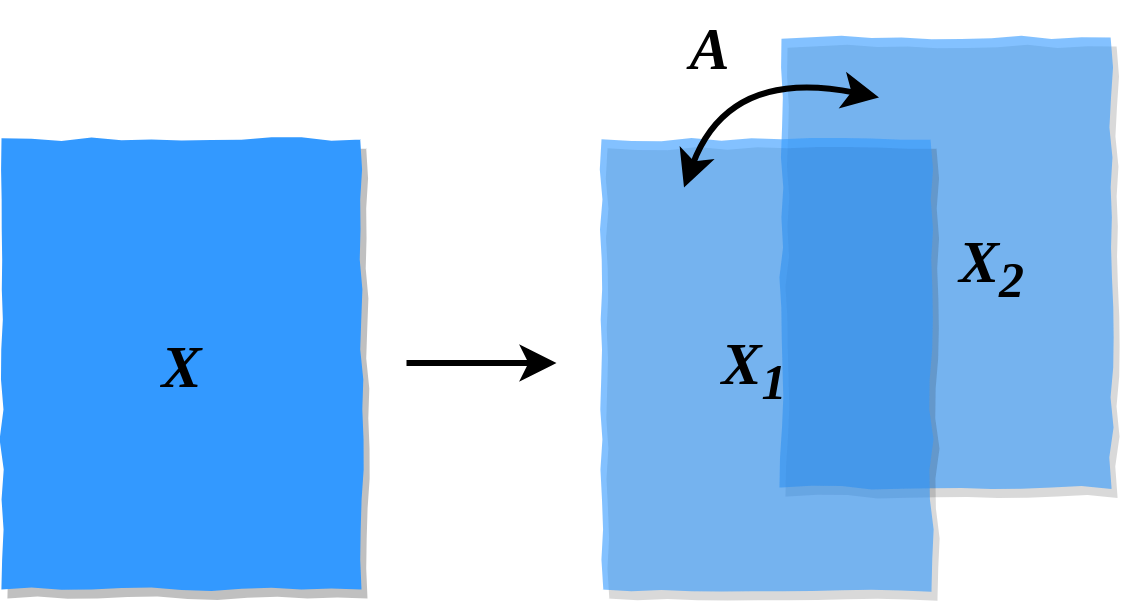
\includegraphics[width=5.5cm]{data-split.png}
\caption{Spliting the data matrix into \textit{past} and \textit{future} matrices $\bm{X_1}$ and $\bm{X_2}$, linked by the linear operator $\bm{A}$.}
\label{fig:linear_system}
\end{figure}

Note here, that for nonlinear systems, a matrix that transforms $\vec{x}_1$ to $\vec{x}_2$ is different from a matrix that transforms $\vec{x}_2$ to $\vec{x}_3$ and so on. DMD assumes, however, that there is one matrix $\bm{A}$ that does all these transformations at once, with the least amount of error. It finds the \textit{best-fit} linear dynamical system for the non-linear data set. In mathematical terms, we are looking for such $\bm{A}$ that:

\begin{equation} \label{eq:linear_dynamics}
\bm{X_2} = \bm{A} \bm{X_1}
\end{equation}

To solve such system we multiply both sides by the \textit{pseudo-inverse} of matrix $\bm{X_1}$ which we denote by $\bm{X_1}^{+}$:

\begin{equation} \label{eq:linear_dynamics_A}
\bm{A} = \bm{X_2} \bm{X_1}^{+}
\end{equation}

The pseudo-inverse described here, also known as the Moore-Penrose inverse\footnote{Check appendix \ref{app:B} for more information.}, is computed using the least squares method. There is therefore certain information lost when going from eq.(\ref{eq:linear_dynamics}) to eq.(\ref{eq:linear_dynamics_A}).

Once we have solved for matrix $\bm{A}$, we can go back to eq.(\ref{eq:eigenvalue_solution}) and solve for eigenvalues and eigenvectors.

Up to this point, this is what the \textbf{exact DMD} computes. There is however a problem that the eq.(\ref{eq:linear_dynamics_A}) may pose when numerics are involved and this will be addressed in the next section. 

\subsection{Going low-rank}

Matrices $\bm{X_1}^{+}$ and $\bm{X_2}$ typically represent huge spacial dimensionality\footnote{This is often the case for data sets where we have very few snapshots in time but a large number of spacial points where the measurements were taken. Graphically, we might think of those matrices as being "tall" and this is illustrated in Figure \ref{fig:data-matrix}.} which in turn means that the matrix $\bm{A}$ can become a square matrix of a massive size. 

\begin{wrapfigure}{R}{0.2\textwidth}
\centering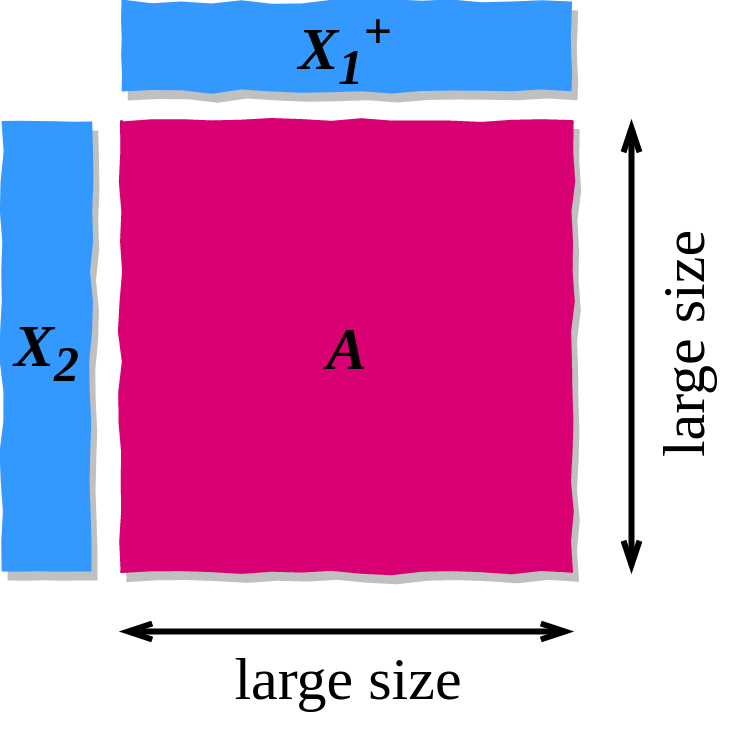
\includegraphics[width=3.5cm]{getting-A.png}
\caption{Building the linear operator $\bm{A}$ in exact DMD.}
\label{fig:data-matrix}
\end{wrapfigure}

We are hence reluctant to perform the multiplication of matrices as is stated in eq.(\ref{eq:linear_dynamics_A}). 

The hope comes from the \textit{Singular Value Decomposition} (SVD). We belive that there are low-rank structures hidden in the data set and we are able to reduce the dimensionality of matrix $\bm{A}$ without significant loss of information.

We perform the SVD on matrix $\bm{X_1}$:

\begin{equation} \label{eq:solution}
\bm{X_1} = \bm{U} \bm{\Sigma} \bm{V}^T 
\end{equation}

Based on the rank structure of the matrix $\bm{X_1}$ (one way to get information about the rank structure is to plot the elements from the diagonal of the matrix $\bm{\Sigma}$) we perform a rank-$r$ truncation on the SVD decomposition and approximate the matrix $\bm{X_1}$ by its low-rank (rank-$r$) representation:

\begin{equation} \label{eq:solution-approx}
\bm{X_1} \approx \bm{X_{1r}} = \bm{U_r} \bm{\Sigma_r} \bm{V_r}^T 
\end{equation}

The pseudo-inverse of the truncated matrix is:

\begin{equation} \label{eq:pseudo-inverse}
\bm{X_{1r}}^{+} = \bm{V_r}  \bm{\Sigma_r}^{-1} \bm{U_r}^T
\end{equation}

The usefulness of this decomposition might not yet be evident, since the matrix $\bm{X_{1r}}$ is of the same size as matrix $\bm{X_{1}}$, they only differ by rank. The idea is to nevertheless use the SVD decomposition but also, to generate a matrix similar to the matrix $\bm{A}$ (since similar matrices share eigenvalues and eigenvectors, among some other properties) but one that will have a smaller size (in fact, it will be size $(r \times r)$). This similar matrix will be denoted $\underline{\bm{A}}$. Since it has a lower size than the original matrix $\bm{A}$, we will only retrieve $r$ eigenvectors and eigenvalues.

\begin{wrapfigure}{R}{0.25\textwidth}
\centering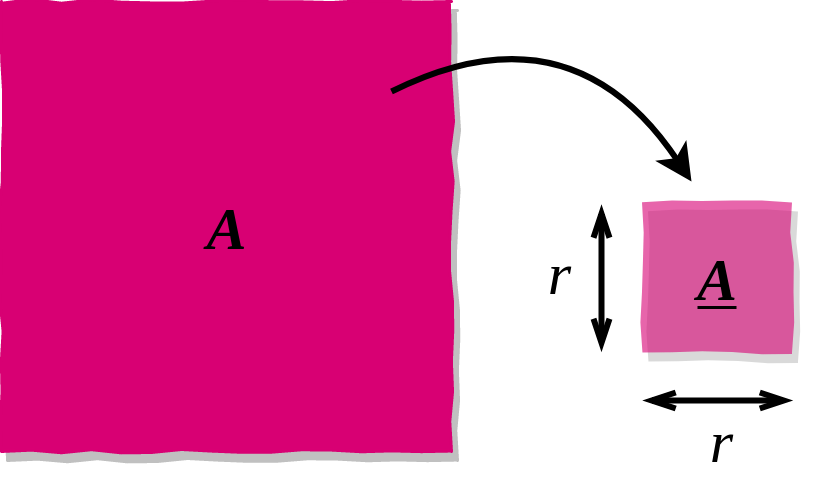
\includegraphics[width=4cm]{similar-matrices.png}
\caption{Similarity transform of matrix $\bm{A}$ to reduce the size.}
\label{fig:similar-matrices}
\end{wrapfigure}

What will now follow are clever mathematical steps performed to avoid computation of the large matrix $\bm{A}$.

We come back to the eq.(\ref{eq:linear_dynamics_A}) and

We perform a \textit{similarity transform} of the matrix $\bm{A}$:

\begin{equation} \label{eq:similarity-transform}
\underline{\bm{A}} = \bm{U_r}^T \bm{A} \bm{U_r}
\end{equation}

Matrix $\bm{A}$ can be written as:

\begin{equation} \label{eq:A}
\bm{A} = \bm{X_2} \bm{V_r} \bm{\Sigma_r}^{-1} \bm{U_r}^T
\end{equation}

The similar matrix $\underline{\bm{A}}$ can be written as:

\begin{equation} \label{eq:A_underline}
\underline{\bm{A}} = \bm{U_r}^T \bm{X_2} \bm{V_r} \bm{\Sigma_r}^{-1} 
\end{equation}

taking into account that $\bm{U_r}^T \bm{U_r} = \bm{I}$.

We have thus chosen a low-dimensional subspace by performing rank-$r$ truncation in which we now find the solution to the linear dynamical system presented initially. The model for the solution is built in this low-dimensional subspace.

\subsection{Eigendecomposition}

Now that we have computed the similar matrix $\underline{\bm{A}}$, 







\subsection{Going back to the original dimensions}

Once the model has been built in the low-dimensional subspace, we want to move to the original dimensions. The DMD modes are obtained from:

\begin{equation} \label{eq:A_underline}
\bm{\Phi} = \bm{X_2} \bm{V} \bm{\Sigma}^{-1} \bm{W}
\end{equation}

DMD modes are not orthogonal. This creates a great capacity of DMD to be applicable to systems where data structure does not exhibit orthogonality.

The solution to the original dynamical system is finally computed:

\begin{equation} \label{eq:x-solution-matrix}
\vec{x}(t) = \bm{\Phi} e^{\bm{\Omega} t} \vec{b}
\end{equation}

the above equation is equivalent to:

\begin{equation} \label{eq:x-solution-summation}
\vec{x}(t)  = \sum_{k=1}^{r} \phi_k e^{\omega_k t} b_k
\end{equation}

\section{A broader view on DMD} \label{sec:view}

What can go wrong with our data sets?

\subsection{Optimized DMD}

- varying time steps

We mentioned earlier, that 

\subsection{Robust DMD}



Sparse Identification


\section{Python example}



\appendix

\section{Solution to linear dynamical systems} \label{app:A}

We first recall the general solution to the differential equation:

\begin{equation} \label{eq:DE_exp}
\frac{d f(x)}{dt} = f(x)
\end{equation}

to be the exponential function: $f(x) = a \cdot e^{x}$.


In an analogous way, the general solution to the linear dynamical system of the form:

\begin{equation} \label{eq:system_linear_A}
\frac{d \vec{x}}{dt} = \bm{A} \vec{x}
\end{equation}

is:

\begin{equation} \label{eq:general_solution_A}
\vec{x} = \vec{v} e^{\bm{\lambda} t}
\end{equation}

Computing the time derivative of the eq. \ref{eq:general_solution_A} we get:

\begin{equation} \label{eq:sub1}
\frac{d \vec{x}}{dt} = \vec{v} \bm{\lambda} e^{\bm{\lambda} t}
\end{equation}

And substituting the eq. \ref{eq:general_solution_A} to eq. \ref{eq:system_linear_A} we get:

\begin{equation} \label{eq:sub2}
\frac{d \vec{x}}{dt} = \bm{A} \vec{v} e^{\bm{\lambda} t}
\end{equation}

The nontrivial solution for the equality of these two above equations is obtained when:

\begin{equation} \label{eq:eigval}
\bm{A} \vec{v} = \bm{\lambda} \vec{v} 
\end{equation}

which is the statement of eigenvalue problem.



\begin{figure}[H]
\centering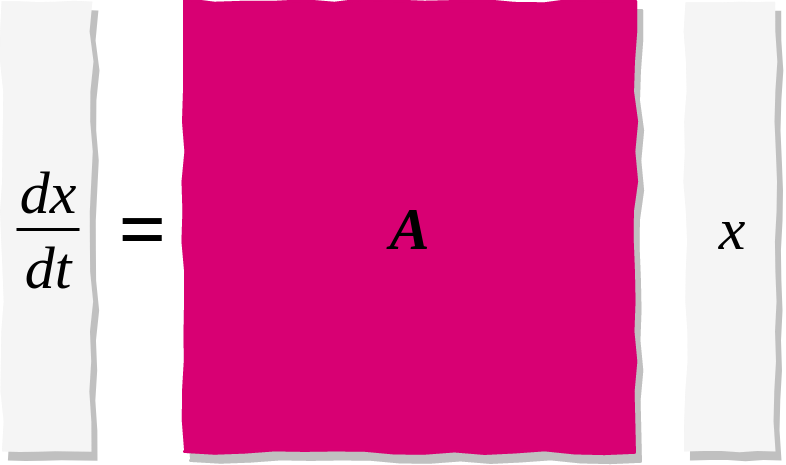
\includegraphics[width=5cm]{lin-dyn.png}
\caption{Linear dynamical system.}
\label{fig:linear_system}
\end{figure}










\section{Moore-Penrose inverse} \label{app:B}




\section{Singular Value Decomposition} \label{app:C}


\begin{figure}[H]
\centering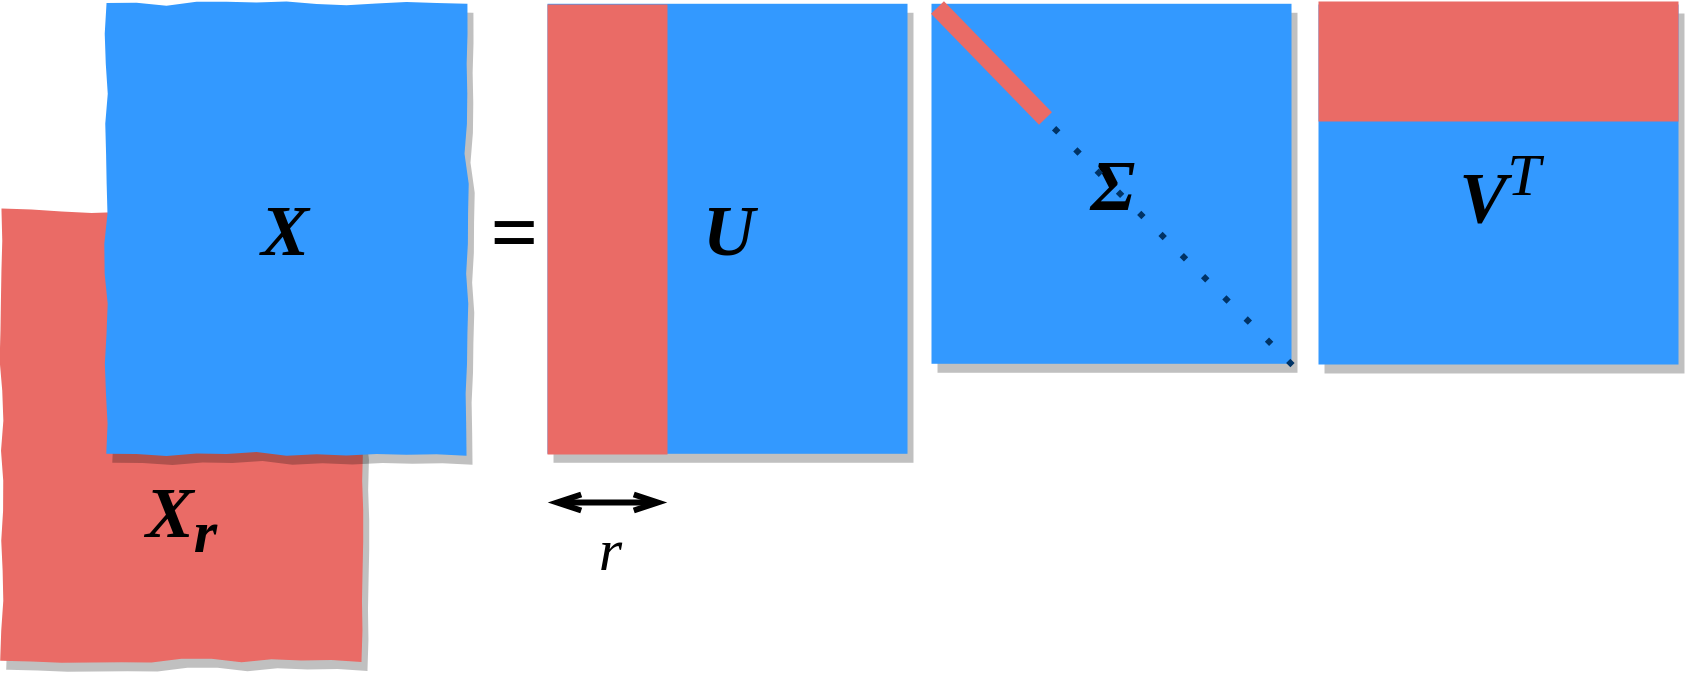
\includegraphics[width=8cm]{svd.png}
\caption{Sizes of component matrices in the Singular Value Decomposition and after rank truncation.}
\label{fig:linear_system}
\end{figure}


\thebibliography{}

\bibitem{Prof_Nathan_Kutz} N. Kutz, \textit{Dynamic Mode Decomposition Theory}, an online lecture: https://youtu.be/bYfGVQ1Sg98 \label{bib:kutz_1}

\bibitem{Prof_Nathan_Kutz} N. Kutz, \textit{Dynamic Mode Decomposition Code }, an online lecture: https://youtu.be/KAau5TBU0Sc \label{bib:kutz_2}

\bibitem{Prof_Edward_Scheinerman} E. R. Scheinerman, \textit{Invitation to Dynamical Systems}

\bibitem{Prof_Gilbert_Strang} G. Strang, \textit{Introduction to Linear Algebra}, 5th edition

\bibitem{} K. Zdybal, The von Karman Institute for Fluid Dynamics: \textit{POD and DMD decomposition of numerical and experimental data}, stagiaire report 

\end{document}
